\documentclass[14pt,a4paper,titlepage]{article}
\usepackage[utf8]{inputenc}
%设置默认语言为德语
\usepackage[ngerman]{babel}
\usepackage{amsmath}
\usepackage{amsfonts}
\usepackage{amssymb}
\usepackage{graphicx}
\usepackage{titlesec}
%\usepackage{lipsum}
\usepackage{setspace}
%设置缩写格式
\usepackage[nohyperlinks, printonlyused, withpage]{acronym}
%设置取消拆分长单词
\usepackage[none]{hyphenat}
%设置对齐方式
\usepackage[document]{ragged2e}
%设置超链接格式
\usepackage{hyperref}
\hypersetup{
	colorlinks=true,
	linkcolor=black,
	filecolor=blue,      
	urlcolor=black,
}

\urlstyle{same}
%设置各个分段的格式
\titleformat{\section}
{\normalfont\Large\bfseries}{\thesection}{1em}{}
\titleformat{\subsection}
{\normalfont\large\bfseries}{\thesubsection}{1em}{}
\titleformat{\subsubsection}
{\normalfont\normalsize\bfseries}{\thesubsubsection}{1em}{}
\titleformat{\paragraph}[runin]
{\normalfont\normalsize\bfseries}{\theparagraph}{1em}{}
\titleformat{\subparagraph}[runin]
{\normalfont\normalsize\bfseries}{\thesubparagraph}{1em}{}
%取消自动缩进
\setlength{\parindent}{0in}
%设置行间距
\linespread{1.213}
\spacing{1.213}
\begin{document}
	%self-made title page
	\begin{titlepage}
		\centering
		
\includegraphics[width=0.5\textwidth]{HSZG.png}\par\vspace{1cm}
		{\scshape\LARGE Hochschule Zittau/Görlitz \par}
		\vspace{1cm}
		{\scshape\Large Praktikumsbeleg\par}
		\vspace{1.5cm}
		{\huge\bfseries Untersuchung und Implementierung von Methoden der CAD-gestützten Roboterprogrammierung\par}
		\vspace{2cm}
		{\large\itshape Dongliang Cao\par}
		\vspace{2cm}
		\begin{minipage}{2.4in}
			{\large Bearbeitungszeitraum \\ Matrikelnummer \\ Betreuer der Ausbildungsfirma \\ Gutachter der Hochschule}
			
		\end{minipage}
		\hfill
		\begin{minipage}{2.0in}
			{\large 3 Monate \\ 
				217043 \\Dr.-Ing. habil. Fan Dai \\
			Prof. Dr. Stefan Bischoff}
		\end{minipage}
		% Bottom of the page
		\vfill
		{\large \today\par}
	\end{titlepage}

	\renewcommand{\abstractname}{Danksagung}

	\begin{abstract}
		
		Ich möchte mich beim Prof. Stefan Bischoff bedanken, dass er mein Betreuer an der Hochschule ist, und mich bei dem Praktikum unterstützt. 
		\bigbreak
		Ich möchte auch Dr. Dai Fan, meinem Betreuer bei ABB Forschungszentrum danken. In meinem Praktikum hat er mir bei theoretischer Fachkenntnisse und auch bei praktischer Anwendungsbereich viele Unterstützung gegeben. Er hat mir alles klar erklärt mit viel Geduld und Verständnis. 
	\end{abstract}
	\renewcommand{\abstractname}{Selbständigkeitserklärung}
	\begin{abstract}
		
		Ich versichere hiermit, dass ich meine Praxisarbeit mit dem Thema „Untersuchung und Implementierung von Methoden der CAD-gestützten Roboterprogrammierung“ selbstständig verfasst und keine anderen als die angegebenen Quellen und Hilfsmittel benutzt habe. Ich versichere zudem, dass die eingereichte elektronische Fassung mit der gedruckten Fassung übereinstimmt.
		\bigbreak
		Die Arbeit wurde bisher keiner anderen Prüfungsbehörde vorgelegt und auch noch nicht veröffentlicht.
		\vfill
		\begin{minipage}{2.0in}
			{\large \underline{Mannheim, \today}
			\\ Ort, Datum}
		\end{minipage}
		\hfill
		\begin{minipage}{2.0in}
			{\large \underline{\hspace{3cm}Dongliang Cao}
				\\ Unterschrift}
		\end{minipage}
	\end{abstract}
	\tableofcontents
	\pagebreak
	\section{Einführung}
	\subsection{Problemstellung}
		Die zunehmende Komplexität von Produkten und Maschinen sowie kurze Produktionszyklen bei kleinen Losgrößen stellen die Industriebranche vor große Herausforderungen. Sowohl die Programmierung von Industrierobotern im Online-Modus mit Handbediengerät als auch im Offline-Modus mit virtueller Simulation erfordert spezielle Kenntnisse in der Robotik und in fertigungsabhängigen Robotersteuerungssystemen und ist bei komplizierten Aufgaben sehr zeitaufwändig. Insbesondere klein- und mittelständische Unternehmen konfrontieren mit zusätzlichen Hindernissen wie höhe Investitionen für die Ausbildung der nicht qualifizierten Mitarbeitern und die wegen der Inbetriebnahme von Roboterzeller verlängerten Produktionszyklen.   
	\subsection{Motivation}
		Um die Ingenieuren von den wiederholenden, eintönigen und zeitaufwändigen Programmierungsverfahren zu befreien und deshalb sich mehr auf das Projekt selbst und dessen notwendigen Operationen zu konzentrieren, benötigt neue Methode für die Erzeugung des Roboterprogrammes, die effizienter, intuitiver und benutzerfreundlicher ist. 
		\bigbreak
		Grundsätzlich gesagt, im Vergleich mit Online Programmierung kann \acs{olp} dank der Simulationsumgebung mehr Zeit und Bemühung für Benutzer sparen. Der Benutzter braucht nicht vor Ort den echten Roboter zu steuern, um die gewünschte Position zu erreichen und selbst zu programmieren, sondern sitzt sich vor den Bildschirm im Büro und gebt die notwendigen Positionen, Konfigurationen und Befehle in Simulationsumgebung. Nach der Simulation, die die Erreichbarkeit der gewünschten Positionen und die Kollisionsmöglichkeit überprüft, generiert das Roboterprogramm automatisch. Aber der Mangel für heutige Offline-Software ist auch eindeutig, wenn der Benutzer eine lange Reihe von Bewegungsanweisungen definieren möchten, braucht er entweder viele Zeit, um jede Position zu definieren oder weißt er nicht genaue die Positionen. 
		\bigbreak
		Die meiste Information über die wichtigsten Positionen für die Bewegungsanweisung beinhaltet normalerweise das Objekt, das direkt von dem Roboter bedient wird. Und die Information über das Objekt kann durch die Analyse der dahinter versteckten geometrische Daten nachzuziehen. Leider ziehen jetzt wenige Ansätze für die Kombination von CAD-Daten und Offline Programmierung.
		\bigbreak
		Aus obigen Gründen möchte ich in meinem Praktikum ein Add-In-Programm in Robotstudio entwickeln und ermöglicht die automatisch Erzeugung der Position für den Einschub von 2 Objekte. 
		\begin{figure}[h!]
			\centering
			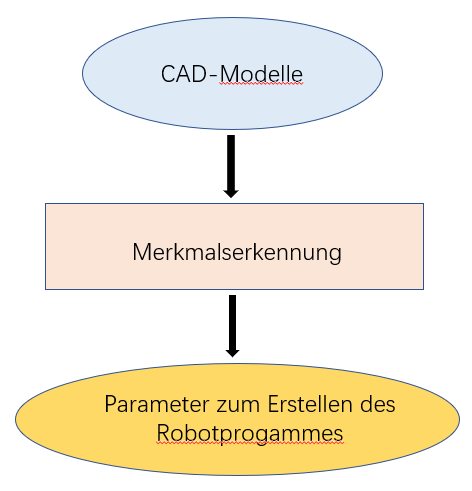
\includegraphics[width=0.5\textwidth]{Bearbeitungsverfahren.png}
			\caption{Bearbeitungsverfahren für CAD-Daten}
			\label{fig1}
		\end{figure}
	\subsection{Zielstellung}
	\paragraph{Extraktion und Analyse der Information von CAD-Daten}
	
	Abruf und Analyse der geometrischen Informationen und Topologieinformationen des Objekts aus der CAD-Datei
	\paragraph{Filtern der Information von CAD-Daten}

	Ausschluss der irrelevanten Informationen und Herausfiltern der Informationen, die Beziehungen zwischen Objekten enthalten
	
	\paragraph{Feststellung der Einschubrichutung und des Einschubabstandes}
	Kalkulation und Bestimmung der potentiellen Einschubrichtungen mithilfe von gefilterten geometrischen Informationen und Topologieinformationen  
	
	\paragraph{Visualisierung der Ergebnisse}
	Visualisierung der Ergebnisse in Benutzeroberfläche
	\pagebreak
	\section{Theoretische Grundlangen}
	\subsection{Offline Programmierung}
	\subsubsection{Definition}
	Die \acf{olp} ist eine Roboterprogrammierungsmethode, bei der das Roboterprogramm unabhängig von der eigentlichen Roboterzelle erstellt wird. Das Roboterprogramm wird dann zur Ausführung auf den realen Industrieroboter hochgeladen. Bei der Offline-Programmierung wird die Roboterzelle durch ein grafisches 3D-Modell in einem Simulator dargestellt. Heutzutage helfen OLP Roboterintegratoren dabei, die optimalen Programm für den Roboter zu erstellen, um eine bestimmte Aufgabe auszuführen. Bei der Simulation des Roboterprogramms können Roboterbewegungen, Erreichbarkeitsanalysen, Kollisions- und Beinahe-Erkennung sowie Zykluszeitberichte berücksichtigt werden.\cite{offline-programming}
	\bigbreak
	\paragraph*{Vorteile}
	\begin{itemize}
		\item [1)]
		Die Offline-Programmierung bricht die Produktion nicht ab, weil das Programm für den Roboter außerhalb des Produktionsprozesses auf einem externen PC geschrieben wird.
		\item[2)]
		Integratoren und Endbenutzer können beim Entwurf einer Arbeitszelle Zeit und Geld sparen im Vergleich mit Online-Programmierung.
		\item[3)]
		Die Fähigkeit zu analysieren, wie sich eine Arbeitszelle verhält, bevor Zeit und Geld in Geräte investiert werden, sorgt für eine reibungslose Umsetzung vom Konzept zur Realität.
	\end{itemize}
	\paragraph{Vorgehensweise mit \acl{olp}}
	\begin{itemize}
		\item[1)]
		\textbf{Erstellung der Arbeitszelle}
		\linebreak
		Eine Arbeitszelle bzw. Roboterzelle bezieht sich auf eine Kombination von einem oder mehreren Robotern und das damit verbundene Werkzeuge, andere Werkstücke und Vorrichtungen. Wenn man eine Arbeitszelle erstellt, soll man zuerst alle Komponente in der Arbeitszelle importieren und danach platzieren. Außerdem muss der Roboter mit einer virtuellen Steuerung verbinden, um zu programmieren.Ein Werkzeug ist ein spezielles Objekt (z. B. eine Lichtbogenschweißzange oder
		ein Greifer), das an einem Werkstück arbeitet. Für korrekte Bewegungen in
		Roboterprogrammen müssen die Parameter des Werkzeugs in den Werkzeugdaten
		angegeben werden. Der wesentliche Teil der Werkzeugdaten ist der \acf{tcp}.
		
		\item[2)] 
		\textbf{Programmierung von Robotern}
		\linebreak
		 Bevor der Benutzer ein Programm für seinen Roboter erstellen, solltet er die vorher genannte Arbeitszelle
		 einrichten, in der sein Roboter arbeiten soll, einschließlich der Roboter, Werkzeug
		 und Vorrichtungen.
		 \bigbreak
		 das Verfahren für die Programmierung von Robotern kann sich hauptsächlich in 5 Schritte unterteilen.
		 \begin{itemize}
		 	\item Erstellen von Positionen
		 	und Bahnen
		 	\item Prüfung der Positionsorientierung und Erreichbarkeit
		 	\item Synchronisieren des Programms
		 	mit der virtuellen
		 	Steuerung
		 	\item Ausführen von textbasierter
		 	Bearbeitung
		 	\item Kollisionserkennung
		 \end{itemize} 
	 	\item[3)]
	 	\textbf{Simulieren von Programmen}
	 	\linebreak
	 	Mit Simulationen werden vollständige Roboterprogramme auf einer virtuellen Steuerung ausgeführt.Durch Simulation kann die Zykluszeit berechnet,die Kollision erkannt, die E/A-Signale simuliert und auch die Ereignisse (Aktion mit einem Trigger verbunden) behandelt werden, um festzustellen, ob das Robotersystem die Erwartung von Endbenutzer erfüllt.
	 	
	 	\item [4)]
	 	\textbf{Aufladung des Programmes in realer Steuerung}
	 	\linebreak
	 	Wenn die Simulation erfolgreich durchgeführt wird, kann der Benutzer das automatisch generiert Programm von Computer in realen Roboter aufladen.   
	\end{itemize}
	\subsubsection{Robotstudio}
	Robotstudio ist ein typisches Anwendungsbeispiel für die \acf{olp}, das von ABB entwickelt und unterstützt wird. RobotStudio ermöglicht der Benutzer das Arbeiten mit einer Offline-Steuerung. Dabei
	handelt es sich um eine virtuelle IRC5-Steuerung, die lokal auf dem PC ausgeführt
	wird. RobotStudio basiert auf dem so genannten Virtual Controller, einer exakten Kopie der Originalsoftware, die den Roboter in Produktionsprozessen steuert. So sind realistische Simulationen möglich, denn zum Einsatz kommen die Daten und Konfigurationen, die auch in der realen Produktion zum Einsatz kommen.\cite{robotstudio} 
	In meiner Arbeit, wird Robotstudio als eine Benutzeroberfläche zur Interaktion und Visualisierung von generierten Ergebnissen bedient. Außerdem wird Robotstudio \acf{sdk} als Programmbibliothek unter .NET Framework für die Entwicklung des Add-In-Programmes verwendet.
	\begin{figure}[h!]
		\centering
		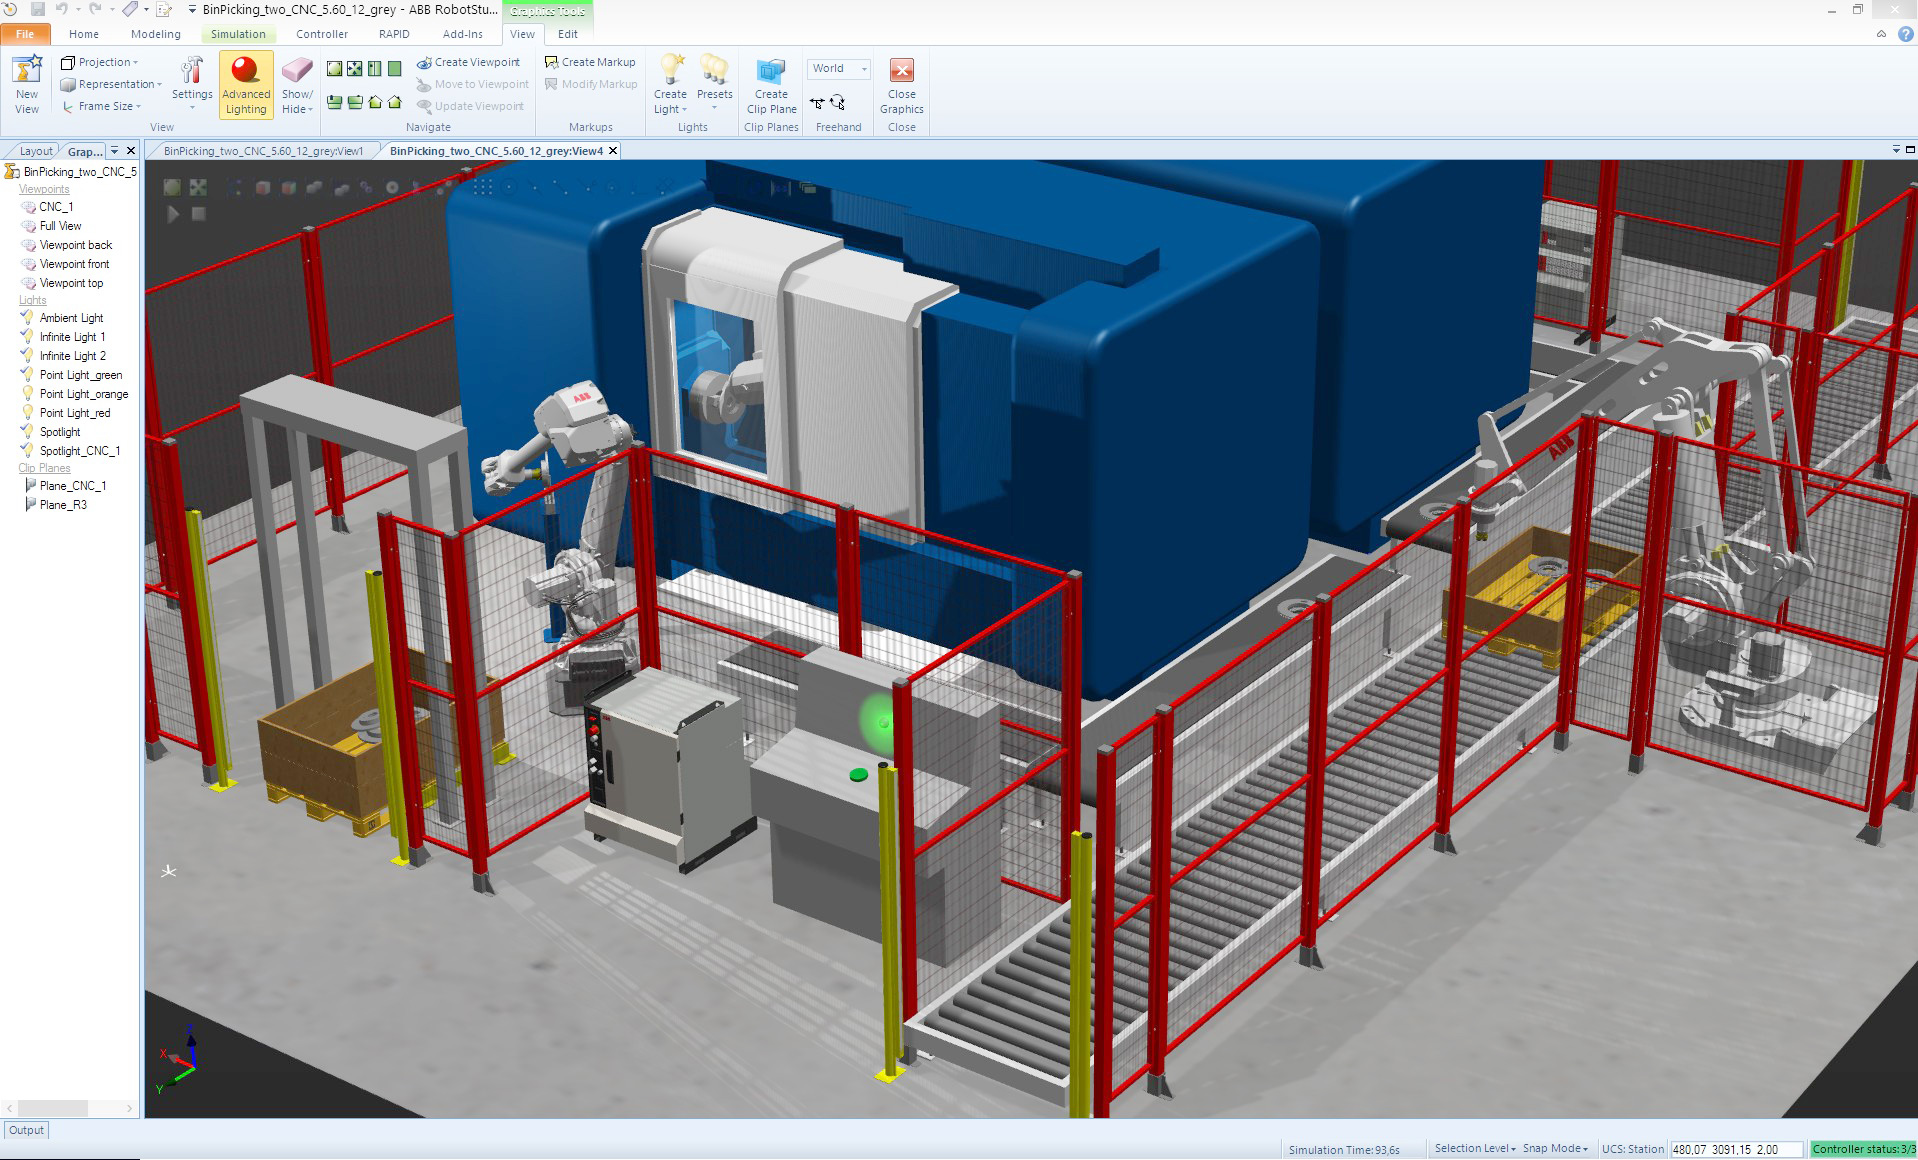
\includegraphics[width=0.8\textwidth]{robotstudio.jpg}
		\caption{Roboterzelle in Robotstudio}
		\label{fig2}
	\end{figure} 
	\pagebreak 
	\subsection{Geometrie und Topologie}
		Geometrie und Topologie sind zwei wichtigste Begriffe für die mathematische Darstellung der räumlichen Information von Objekte in der realen Welt. Die Geometrie bezieht sich in diesem Artikel besonders auf die euklidische Geometrie, die sich mit Punkten, Geraden, Ebenen, Abständen, Winkeln usw. beschäftigt, sowie diejenigen Begriffsbildungen und Methoden, die im Zuge einer systematischen und mathematischen Behandlung dieses Themas entwickelt wurden.\cite{geometrie}Neben der mathematischen Beschreibung der räumlichen Lage und Form von einzelnen Komponenten, beschreibt die Topologie die Lagebeziehung zwischen Geoobjekten, wie z.B. die Knoten, Kante und Masche. In einfachen Systemen entsprechen den Punkten die Knoten, den Linien die Kanten und den Flächen die Maschen.\cite{topologie}
		
		\bigbreak
		Im meisten CAD-Datei wird \acf{b-rep}, auf deutsch Begrenzungsflächenmodell, als Modellierungsform eines Flächen- oder Volumenmodells verwendet. Ein typisches Beispiel: Eine Fläche ist ein begrenzter Teil einer Oberfläche. Eine Kante ist ein begrenzter Teil einer Kurve und ein Scheitelpunkt liegt an einem Punkt. In der Welt des Datenaustauschs definiert \acf{step} auch einige Datenmodelle für \acs{b-rep}. Die allgemeinen generischen topologischen und geometrischen Modelle sind in der geometrischen und topologischen Darstellung nach ISO 10303-42 definiert.\cite{b-rep}
		    
	\subsubsection{Geometrie}
		Die Geometrie, die für die Modellierung von Geoobjekte in CAD-System, handelt sich um euklidische Geometrie. Die Geometrie kann sich in vier Kategorien einteilen.
		\begin{itemize}
			\item[1)]
			\textbf{Punkten}, die in einem dreidimensionalen Raum existieren.
			\linebreak
			Der Punkt ist das grundlegendste geometrische Konzept in einem Raum. Ein Punkt im dreidimensionalen Raum wird normalerweise in einem kartesischen Koordinatensystem als eine Position dargestellt und die Position enthält drei Werte, die sich auf x, y, z-Koordinaten beziehen. 
			\bigbreak
			\emph{Hinweis:}
			\linebreak
			{\small Der Punkt in einem dreidimensionalen Raum kann nicht nur eine Position, sondern auch einen dreidimensionalen Vektor repräsentieren. Ein Vektor ist als eine räumliche Verschiebung von einer Position zu einer anderen Position zu definieren.}    
			\item[2)] 
			\textbf{Kurven}, die in einem dreidimensionalen Raum existieren.
			\linebreak
			In der Mathematik ist eine Kurve ein eindimensionales Objekt. Eindimensional bedeutet dabei informell, dass man sich auf der Kurve nur in einer Richtung (bzw. der Gegenrichtung) bewegen kann. Ob die Kurve in der zweidimensionalen Ebene liegt („ebene Kurve“) oder in einem höherdimensionalen Raum.\cite{kurve}
			\bigbreak
			In CAD-System kann sich die Kurve wesentlich aus zwei Gruppe einteilen: analytische Kurve und interpolierte Kurve.
			Alle analytischen Kurven werden von einem Parameter, der normalerweise als t genannt wird, parametrisch dargestellt. Die drei wichtigsten Typen in analytische Kurven sind Geraden, Ellipsen (einschließlich Kreise) und Helices.
			
			\begin{itemize}
				\item \emph{Geraden}
				\\
				Eine Gerade wird durch einen Punkt \(\vec{p_0}\) und eine Richtung \(\vec{r}\) dargestellt. Eine Gerade kann eine unendliche gerade Linie, eine teilweise begrenzte gerade Linie (ein Strahl) oder eine begrenzte gerade Linie (ein Liniensegment) darstellen
				
				\bigbreak
				
				Im dreidimensionalen Raum, die Position eines Punktes auf einer Gerade kann durch die parametrisierte Gleichung berechnet werden.
			    \[ \vec{p(t)} = \vec{p_0} + t\vec{r} \]
			    
				\item \emph{Ellipsen}
				\\
				Eine Ellipse wird durch einen Mittelpunkt \(\vec{p_0}\), einen Einheitsvektor \(\vec{n}\), der senkrecht zur Ebene der Ellipse ist, einen Vektor \(\vec{M}\), der die Hauptachse der Ellipse (einschließlich der Größe der Hauptachse) repräsentiert, und das Radiusverhältnis \(\alpha\) (das Verhältnis der Nebenachsenlänge zur Hauptachsenlänge) vollständig definiert.
				
				\bigbreak
				
				Im dreidimensionalen Raum, die Position eines Punktes auf einer Ellipse kann durch die parametrisierte Gleichung berechnet werden.
				\begin{align*}
				\vec{p(t)} &= \vec{p_0} + \vec{M}\cos{t} + \vec{m}\sin{t}\\
			    \vec{m} &= \alpha(\vec{n}\times\vec{M})		
				\end{align*}
				\begin{figure}[h!]
					\centering
					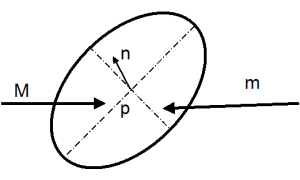
\includegraphics[width=0.5\linewidth]{ellipsen.png}
					\caption{Ellipse}
					\label{fig3}
				\end{figure}
				
				\item \emph{Helices}
				\\
				Eine Helix ist typischerweise eine dreidimensionale Spule, die wie ein Schraubengewinde auf der Oberfläche eines Zylinders liegt.
				Eine Helix wird definiert durch einen Wurzelpunkt, einen Einheitsvektor, der die Achse der Helix definiert, einen Vektor vom Wurzelpunkt zu einem Punkt auf der Kurve, die Steigung, die Drehrichtung und den Parameterbereich.
				
				\bigbreak
				
				Im dreidimensionalen Raum, die Position eines Punktes auf einer Helix kann durch die parametrisierte Gleichung berechnet werden.
				\[ \vec{p(t)} = a\cos{t}\vec{x_0} + a\sin{t}\vec{y_0} + bt\vec{z_0}\]
				
				\begin{figure}[h!]
					\centering
					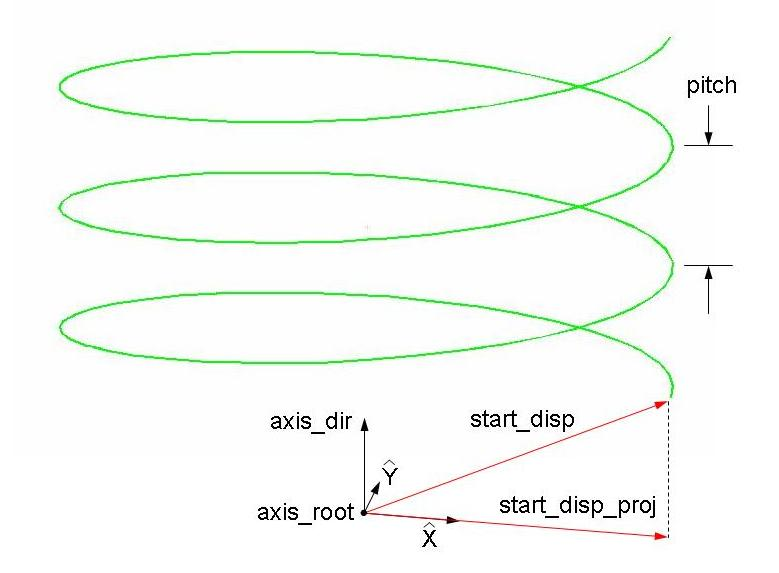
\includegraphics[width=0.4\linewidth]{helix.png}
					\caption{Helix}
					\label{fig4}
				\end{figure}
			\end{itemize}
			\item[3)]
			\textbf{Oberflächen}, die in einem dreidimensionalen Raum existieren.
			\\
			Der Begriff Oberfläche hat mehrere Bedeutungen. In CAD-System wird dieser Begriff am häufigsten in seinem geometrischen oder mathematischen Sinne verwendet, um ein zweidimensionales Objekt in einem dreidimensionalen Raum mit einer einzigen geometrischen Definition zu beschreiben.
			\bigbreak
			
				Änlich wie Kurven, in CAD-System kann sich die Oberfläche wesentlich aus zwei Gruppe einteilen: analytische Oberfläche und interpolierte Oberfläche.
				Alle analytischen Oberflächen werden von zwei Parametern, die normalerweise als u, v genannt werden, parametrisch dargestellt. Die vier wichtigsten Typen in analytische Oberflächen sind Ebenen, Kegel, Kugel und Torus.
			
			\begin{itemize}
				\item \emph{Ebenen}
					\\
					In der Geometrie repräsentiert eine Ebene eine unendliche ebene Fläche oder einen begrenzten Bereich auf einer solchen Fläche.
					Der Parameter einer Ebene wird durch einen Punkt und einen Normalenvektor definiert.Die Parametrisierung einer Ebene wird durch zwei zusätzliche Parameter definiert: einen Vektor senkrecht zur Normalen, der die U- Parameterrichtung und Skalierung sowie ein Flag, das angibt, ob die Parametrisierung der Ebene für Rechts- oder Linkshänder erfolgt.
					
					\bigbreak
					Normalerweise, eine Ebene wird in Bezug auf ein rechtshändiges Koordinatensystem definiert \( (\vec{U},\vec{V},\vec{N}) \).
					Die Richtung von \( \vec{U}\) ist von der entsprechenden Vector bestimmt und die Richtung von \( \vec{V}\) ist von die Richtung von \( (\vec{N}\times\vec{U}) \) bestimmt.
					
					\begin{equation*}
					\vec{p(u,v)} = \vec{R_0} + u\vec{U} + v\vec{V}
					\end{equation*}
					\begin{figure}[h!]
						\centering
						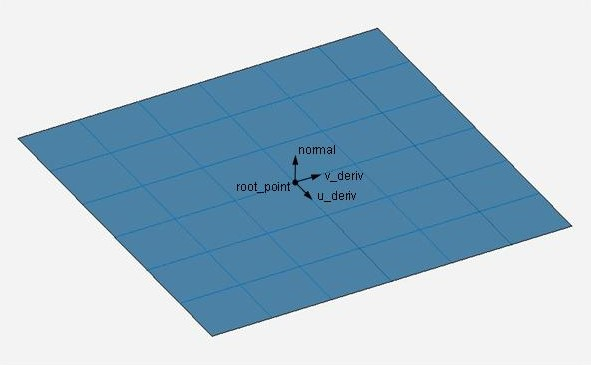
\includegraphics[width=0.5\linewidth]{plane.png}
						\caption{Ebene}
						\label{fig5}
					\end{figure}
				
				\item \emph{Kegel}
					\\
					In der Geometrie, repräsentiert ein Kegel entweder einen Kegel oder einen Zylinder. Die Geometrie eines Kegels wird durch eine Basisellipse und den Sinus und Cosinus des Haupthalbwinkels des Kegels definiert. Die Normale der Basisellipse repräsentiert die Achse des Kegels. 

					\begin{align*}
						x &= au\cos{v}\\
						y &= au\sin{v}\\
						z &= u
					\end{align*}
					\begin{figure}[h!]
						\centering
						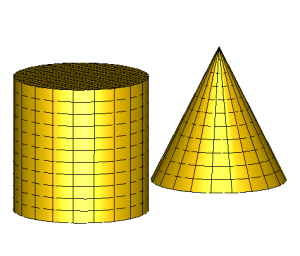
\includegraphics[width=0.5\linewidth]{cone.png}
						\caption{Cone}
						\label{fig6}
					\end{figure}
			\end{itemize}
			
		  
		\end{itemize}
	\subsubsection{Topologie}
		Das Grundkonzept von \acf{b-rep} ist die Topologie, die beschreibt, wie Elemente begrenzt und verbunden werden. Topologie beschreibt die Beziehungen zwischen unterschiedlichen Geoobjekten.
		\bigbreak
		Zum Beispiel, die Topologie kann sagen, dass eine Kante \( E_1 \) durch die Eckpunkte  \( V_1 \) und \( V_2 \) begrenzt ist. Falls wir auch wissen, dass eine andere Kante \( E_2 \), durch die Eckpunkte \( V_2 \) und \( V_3 \) begrenzt ist, dann können wir davon ableiten, dass die Kanten \( E_1 \) und \( E_2 \) benachbart sind, weil \( V_2 \) beide Kanten begrenzt. 
				\begin{figure}[h!]
				\centering
				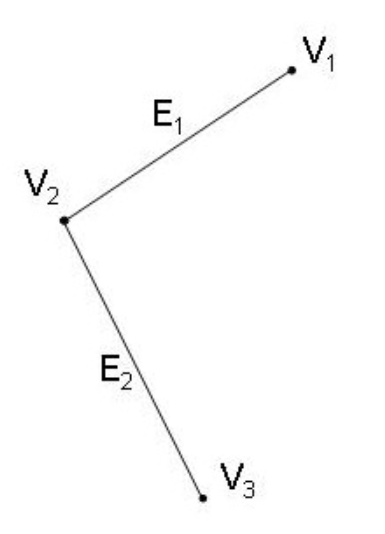
\includegraphics[width=0.25\linewidth]{beispieltopologie.png}
				\caption{Ein Beispiel für die Bedeutung von Topologie}
				\label{fig9}
			\end{figure}
		\pagebreak
		\bigbreak
		Eine typische Hierarchie für die topologische Elementen mit Volumen besteht einerseits aus Body, Lump, Shells, Subshells, Faces, Loops, Coedges, Edges, Vertices, andererseits für die Elemente ohne Volumen existiert keine Faces, sondern Wires.  
			\begin{figure}[h!]
			\centering
			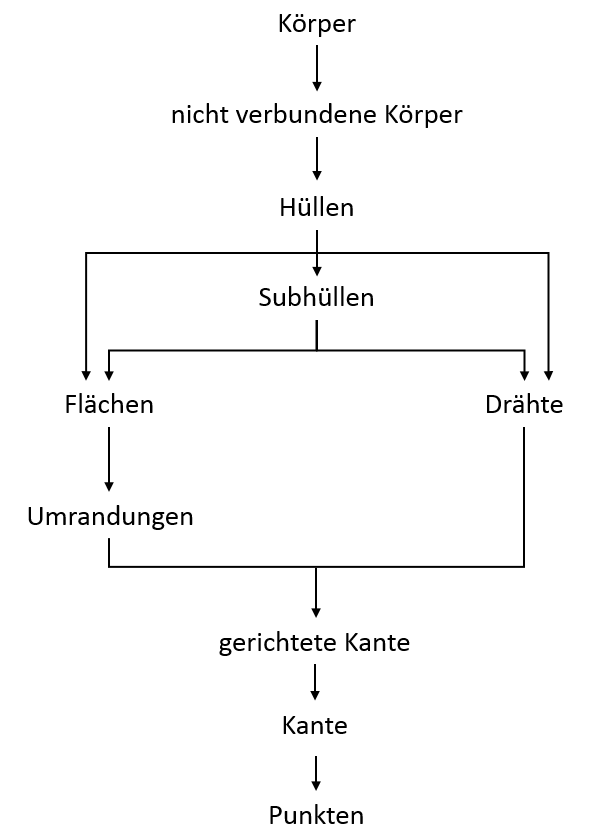
\includegraphics[width=0.5\linewidth]{topology.png}
			\caption{Hierarchische Beziehungen zwischen den topologischen Elementen}
			\label{fig8}
			\end{figure}
	\pagebreak
	\subsection{CAD Modellierung}
		Verschiedene CAD-Software unterstützen unterschiedliche CAD-Dateien. In SolidWorks haben sie beispielsweise proprietäre Formate wie ein Teil, der als ".prt" definiert ist, und eine Baugruppe, die als ".asm" gespeichert ist. Die verschiedenen proprietären CAD-Dateiformate werden von unterschiedlichen CAD-Konstruktionssoftware wie Pro Engineer, SolidWorks und AutoCAD verwendet. Wegen der Vielfalt von CAD-Dateiformat, ein neutrales CAD-Dateiformat, mit dem die Daten zwischen verschiedenen CAD-Programmen ausgetauscht werden können, zu finden, ist für die Einarbeitung der CAD-Datei sehr wichtig.
		\begin{figure}[h!]
			\centering
			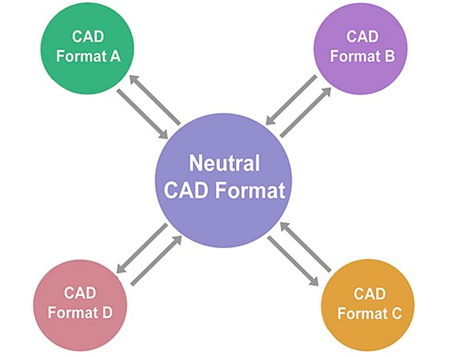
\includegraphics[width=0.5\linewidth]{cad.png}
			\caption{neutrales CAD-Dateiformat hilft Datenaustausch}
			\label{fig7}
		\end{figure}
		\break
		Derzeit eines der beliebtesten CAD-Dateiformat ist \acs{step}.Die Vorteile von \acs{step} spiegelt sich hauptsächlich in den folgenden vier Punkten wieder.
		\begin{itemize}
			\item[1)]
			Ermöglicht das Anzeigen und Ändern von Geometrie mithilfe eines beliebigen CAD-Tools, das STEP-Geometrie interpretieren kann, und unterbricht die Abhängigkeit zwischen CAD-Systemen und Produktdefinition
			\item[2)] 
			Enthält das Assembly-Schema, das alle Connector-Entitäten enthält
			\item[3)] 
			Nützlich zum Gruppieren von mechanischen Elementen in Bestimmte Ansicht
			\item[4)] 
			Einfache Ableitung der impliziten Informationsinhalte. 
		\end{itemize}  
	\section{Aufgabenstellung}
		\subsection{Addin-Entwicklung in Robotstudio}
			Die Entwicklung für die Benutzeroberfläche zur Interaktion und Visualisierung wird mit dem RobotStudio SDK ausgeführt. Hierbei handelt es sich um ein Framework, mit dem die ABB RobotStudio Funktionen über die verfügbaren APIs bearbeitet werden. Die Programmiersprache C\# wird zum Entwickeln der Front-End-Operationen verwendet. 
			Das SDK bietet Visual Studio-Projektvorlagen und APIs zum Erweitern von RobotStudio und zum Erstellen von SmartComponents mit Code-Behind.Download
			
			\bigbreak
			\textbf{\emph{Die Vorgehensweise für die Entwicklung von UI erläutert wie folgendes:}}
			\\
			\begin{itemize}
				\item[1)]
				\textbf{Herunterladen und Installation von RobotStudio SDK} 
				\\
				RobotStudio SDK kann man in die Website \href{http://developercenter.robotstudio.com/downloads_robotstudio}{ABB Developer Center} herunterladen. Bevor man RobotStudio SDK installiert, muss man beachten, dass zuvor Visual Studio 2015/2017 schon am Computer installiert ist. 
				
				\item[2)] 
				\textbf{Erstellung eines neuen Add-in Projektes in Visual Studio}
				\\
				Öffnen Sie zuerst Microsoft Visual Studio und wechseln Sie zu einem neuen Projekt. Aufgrund der Installation von RobotStudio SDK werden in der folgenden Abbildung die folgenden Vorlagen angezeigt.
				Wählen Sie aus der Liste RobotStudio 6.0 Empty Add-In aus und wählen Sie einen Namen für das Projekt.\\
					\begin{figure}[h!]
					\centering
					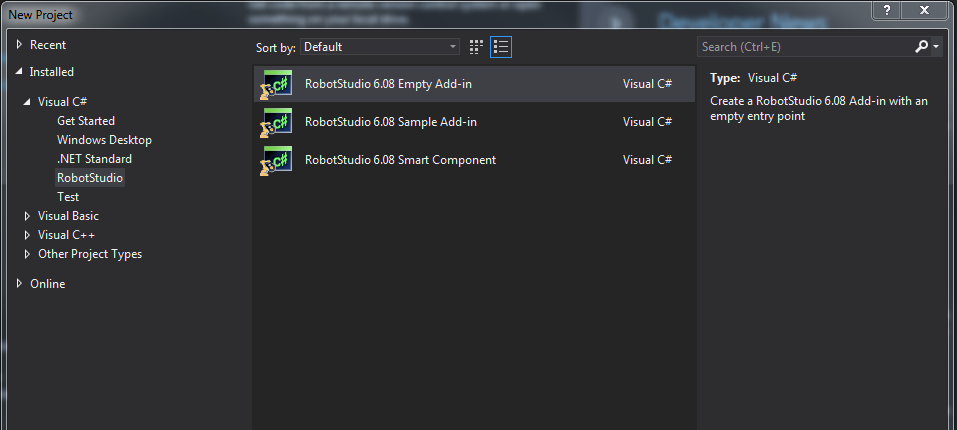
\includegraphics[width=0.8\linewidth]{addin.png}
					\caption{neues Projekt für RobotStudio Add-in auswählen}
					\end{figure}
				Aus dieser Vorlage wird die folgende Lösung mit der * .cs-Datei und den grundlegenden RobotStudio SDK * .dlls generiert, die als Referenz zu dieser Lösung verwendet wurden. Jetzt wird mit der * .sln die Umgebung für die Entwicklung des RobotStudio-Add-Ins festgelegt.\\
					\begin{figure}[h!]
					\centering
					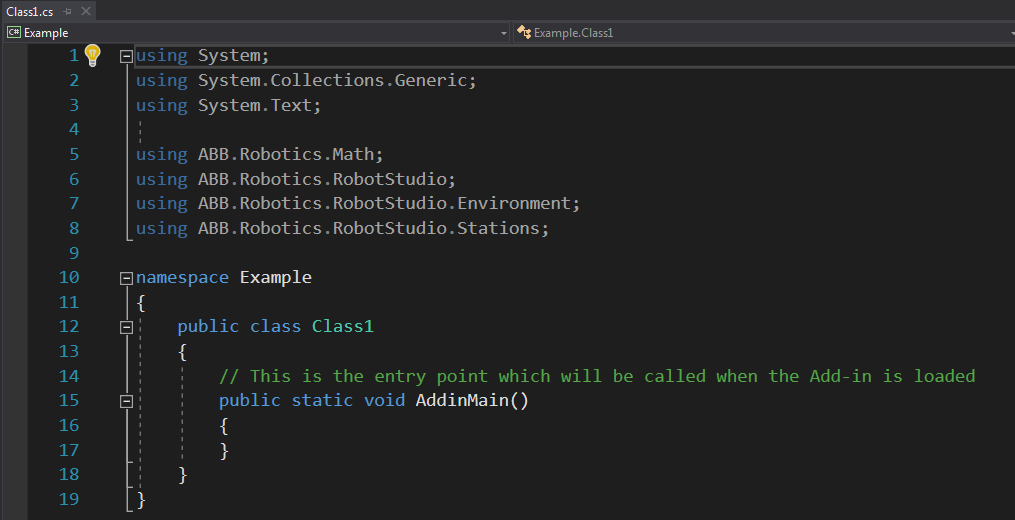
\includegraphics[width=0.8\linewidth]{cs.png}
					\caption{leere Lösung für RobotStudio Add-in}
					\end{figure}
				\bigbreak
				Führen Sie den Build-Befehl in Visual Studio aus, um den Code zu kompilieren und eine .rsaddin-Datei für das Add-In zu generieren. Diese .rsaddin-Datei ist dafür verantwortlich, dass RobotStudio die Add-In-Assembly (die .dll-Datei) lädt.
				\pagebreak
				\item[3)]
				\textbf{UI-Entwicklung}
				\\
				Im RobotStudio-Arbeitsbereich gibt es verschiedene Arten von Bereichen, z.B. Ribbonbereich, Eigenschaftsbereich und Arbeitsbereich.
					\begin{figure}[h!]
						\centering
						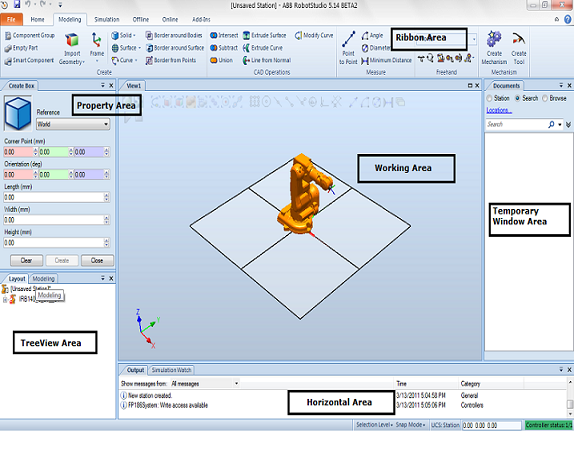
\includegraphics[width=0.8\linewidth]{workarea.png}
						\caption{Arbeitsbereich in RobotStudio}
					\end{figure}
				
				Um sich besser an die Gewohnheit des Benutzers anzupassen, verwende ich den Ribbonbereich und füge ich ein neues RibbonButton hinzu. 
				\bigbreak
				Die Reihfolge für die Hinzufügung des Ribbons ist grundsätzlich wie folgendes:\\
					\begin{figure}[h!]
						\centering
						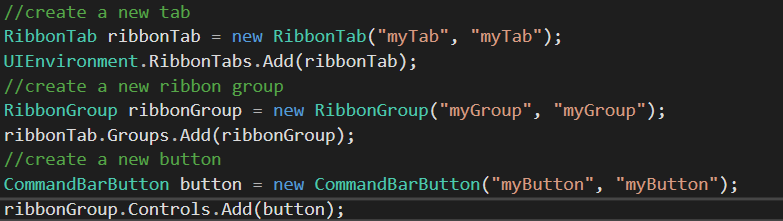
\includegraphics[width=0.8\linewidth]{createbutton.png}
						\caption{Der Kode für die Erstellung von einem Button}
					\end{figure}
				\pagebreak
				\emph{Erstens}, ein neues RibbonTab zu erstellen und in UIEnvironment hinzuzufügen\\
				\emph{Zweitens},
				 ein neues RibbonGroup zu erstellen und in das vorher erstellte RibbonTab hinzuzufügen\\
				\emph{Drittens},
				 ein neues RibbonButton zu erstellen und in das vorher erstellte RibbonGroup hinzuzufügen
				\bigbreak
				Um die Organisation der Kodestruktur zu verbessern und später besser zu verwalten, habe ich für jeden individuellen Button eine neue Klasse erstellt, sodass die Funktionen und die Daten in dieselbe Klasse eingekapselt sind.
				\bigbreak  
				\begin{figure}[h!]
					\centering
					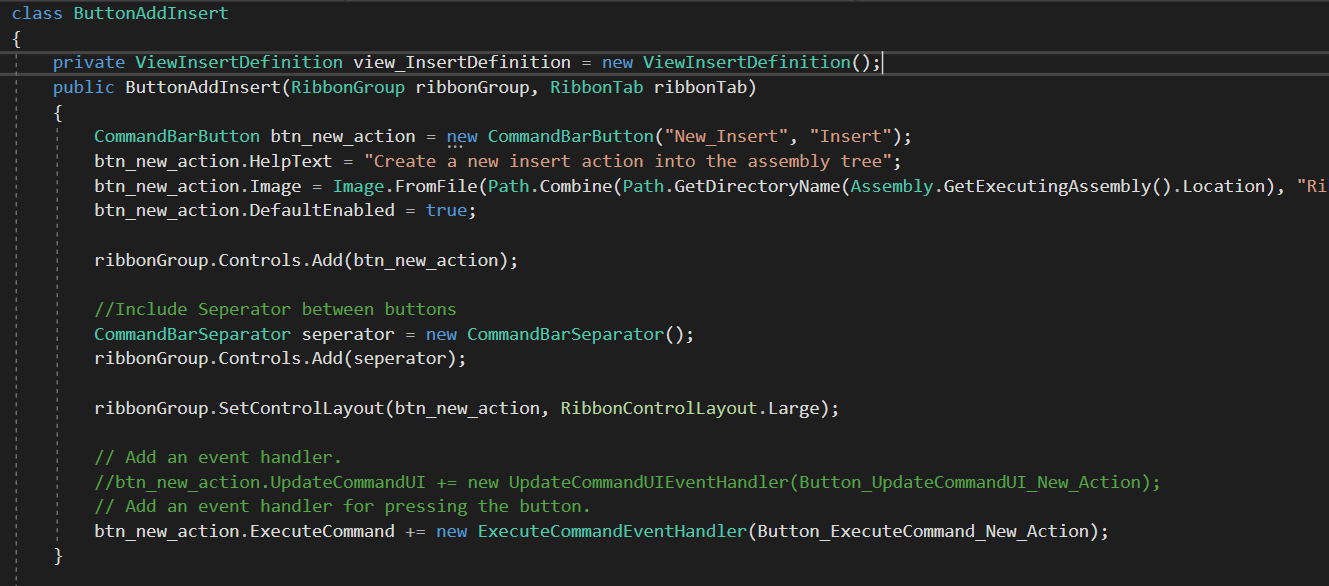
\includegraphics[width=0.8\linewidth]{buttonclass.png}
					\caption{Ein Beispiel für eine Buttonklasse}
				\end{figure}
				ToolWindow ist eine andere wichtige Klasse für die graphische Benutzeroberfläche, die multifunktional als ein einziger Button ist. Ein ToolWindow ist ein Container für andere graphische Kontrolle, somit ist ein ToolWindow vielseitig und leicht erweiterbar.  Eine typische Anwendung für die Nutzung von ToolWindow ist wie folgende Abbildung gezeigt. \\
				\begin{figure}[h!]
					\centering
					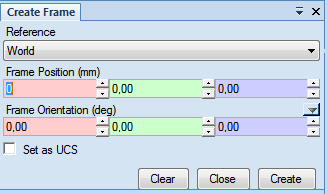
\includegraphics[width=0.8\linewidth]{toolwindow.png}
					\caption{Ein Beispiel für die Anwendung von ToolWindow}
				\end{figure}
				\pagebreak
				Das Beispiel dient zur Erzeugung eines neuen Frames, der als eine relevante Position für anderen Komponenten, wie Roboter, Werkzeug und Bewegungsanweisung usw. bedient. In diesem ToolWindow kann man unterschiedliche graphische Kontrolle sehen, wie ComboBox, Label, NumericTextBox, Button, die als ein Einheit zusammenarbeiten, um die Position und die Orientierung in Bezug auf unterschiedlichen Referenzframen zu bestimmen und endlich zu erzeugen.
			\end{itemize}
			
			
		\subsection{CAD-Modell Analyse Mithilfe von ACIS Modeler}
		\subsection{Einschubrichtungerkennung}
	\section{Methoden}
	\section{Ergebnis und Disskusion}
	\section{Zusammenfassung}
	\section{Ausblick}
	\pagebreak
	\begin{thebibliography}{1}
		\bibitem{offline-programming} 
		\href{https://en.wikipedia.org/wiki/Off-line_programming_(robotics)}{wikipedia:Off-line programming (robotics)}
		
		\bibitem{geometrie}
		\href{https://de.wikipedia.org/wiki/Geometrie}{wikipedia:geometrie}
		
		\bibitem{robotstudio}
		\href{https://new.abb.com/products/robotics/de/robotstudio}{ABB:Offline-Programmierung leicht gemacht!}
		
		\bibitem{topologie}
		\href{https://de.wikipedia.org/wiki/Geodaten#Topologie}{wikipedia:Geodaten}
		
		\bibitem{b-rep}
		\href{https://en.wikipedia.org/wiki/Boundary_representation}{wikipedia: boundary representation}
		
		\bibitem{kurve}
		\href{https://de.wikipedia.org/wiki/Kurve_(Mathematik)}{wikipedia: Kurve (Mathematik)}
	\end{thebibliography}
	\pagebreak
	\listoffigures
	\pagebreak
	\section*{Abkürzungsverzeichnis}
	\begin{acronym}[OLP]
		\acro{olp}[OLP]{Offline-Programmierung}
	\end{acronym}
	\begin{acronym}[TCP]
		\acro{tcp}[TCP]{Werkzeugarbeitspunkt}
	\end{acronym}
	\begin{acronym}[SDK]
		\acro{sdk}[SDK]{Software Development Kit}
	\end{acronym}
	\begin{acronym}[b-rep]
		\acro{b-rep}[b-rep]{boundary representation}
	\end{acronym}
	\begin{acronym}[step]
		\acro{step}[STEP]{the Standard for the Exchange of Product Model data}
	\end{acronym}
\end{document}